\chapter{RStudio: une introduction}
\label{rstudio}

Un environnement de développement intégré (\emph{integrated
  development environment}, IDE) est un progiciel de productivité
destiné au développement de logiciels ou, plus largement, à la
programmation informatique. Il comprend toujours un éditeur de texte
adapté au langage de programmation visé, un environnement de
compilation ou d'exécution du code et, généralement, des outils de
contrôle de versions, de gestion des projets et de navigation dans le
code source.\footnote{%
  À ce compte, GNU~Emacs constitue un environnement de développement
  intégré. Seulement, nous avons davantage insisté sur ses
  fonctionnalités d'éditeur de texte dans ce document.} %

Offert au public depuis 2011, RStudio est le premier environnement
conçu spécifiquement pour l'analyse de données et le développement de
packages avec R. Il est produit par RStudio~Inc.\ et est offert en
version libre ou commerciale, pour une exécution locale
(\emph{desktop}) ou pour un exécution sur un serveur via un navigateur
web.

RStudio occupe aujourd'hui sans conteste la position de tête des
environnements de développement R en matière de convivialité, et ce,
tant pour les débutants que pour les utilisateurs avancés.


\section{Installation}
\label{rstudio:installation}

RStudio est disponible à l'identique pour les plateformes Windows,
OS~X et Linux. Pour une utilisation locale sur son poste de travail,
on installera la version libre (\emph{Open Source}) de RStudio~Desktop
depuis le site
\begin{quote}
  \url{https://www.rstudio.com/products/rstudio/download/}
\end{quote}


\section{Description sommaire}
\label{rstudio:description}

La fenêtre de RStudio se divise toujours en quatre
sous-fenêtres\footnote{%
  Les sous-fenêtres sont appelées en anglais \emph{panes} dans
  l'application.} %
--- sauf au lancement, alors que la sous-fenêtre d'édition de code
source n'est pas visible; voir la \autoref{fig:rstudio:rstudiowindow}.
Dans le sens des aiguilles d'une montre en partant en haut à gauche,
on trouve:
\begin{enumerate}
\item la sous-fenêtre d'édition de code source;
\item le navigateur d'environnement de travail ou d'historique des
  commandes, selon l'onglet sélectionné;
\item le navigateur de fichiers du projet, de packages, de graphiques,
  etc., selon l'onglet sélectionné;
\item la console --- ou ligne de commande --- R.
\end{enumerate}
Au lancement de l'application, la console R occupe toute la gauche de
la fenêtre jusqu'à ce qu'un fichier de code source soit ouvert.

La position des sous-fenêtres dans la grille ne peut être modifiée.
Par contre, chaque sous-fenêtre peut être redimensionnée. De plus, les
onglets des deux navigateurs sont modifiables dans les préférences de
l'application.

\begin{figure}[t]
  %% Capture d'écran et espace additionnel sous l'image
  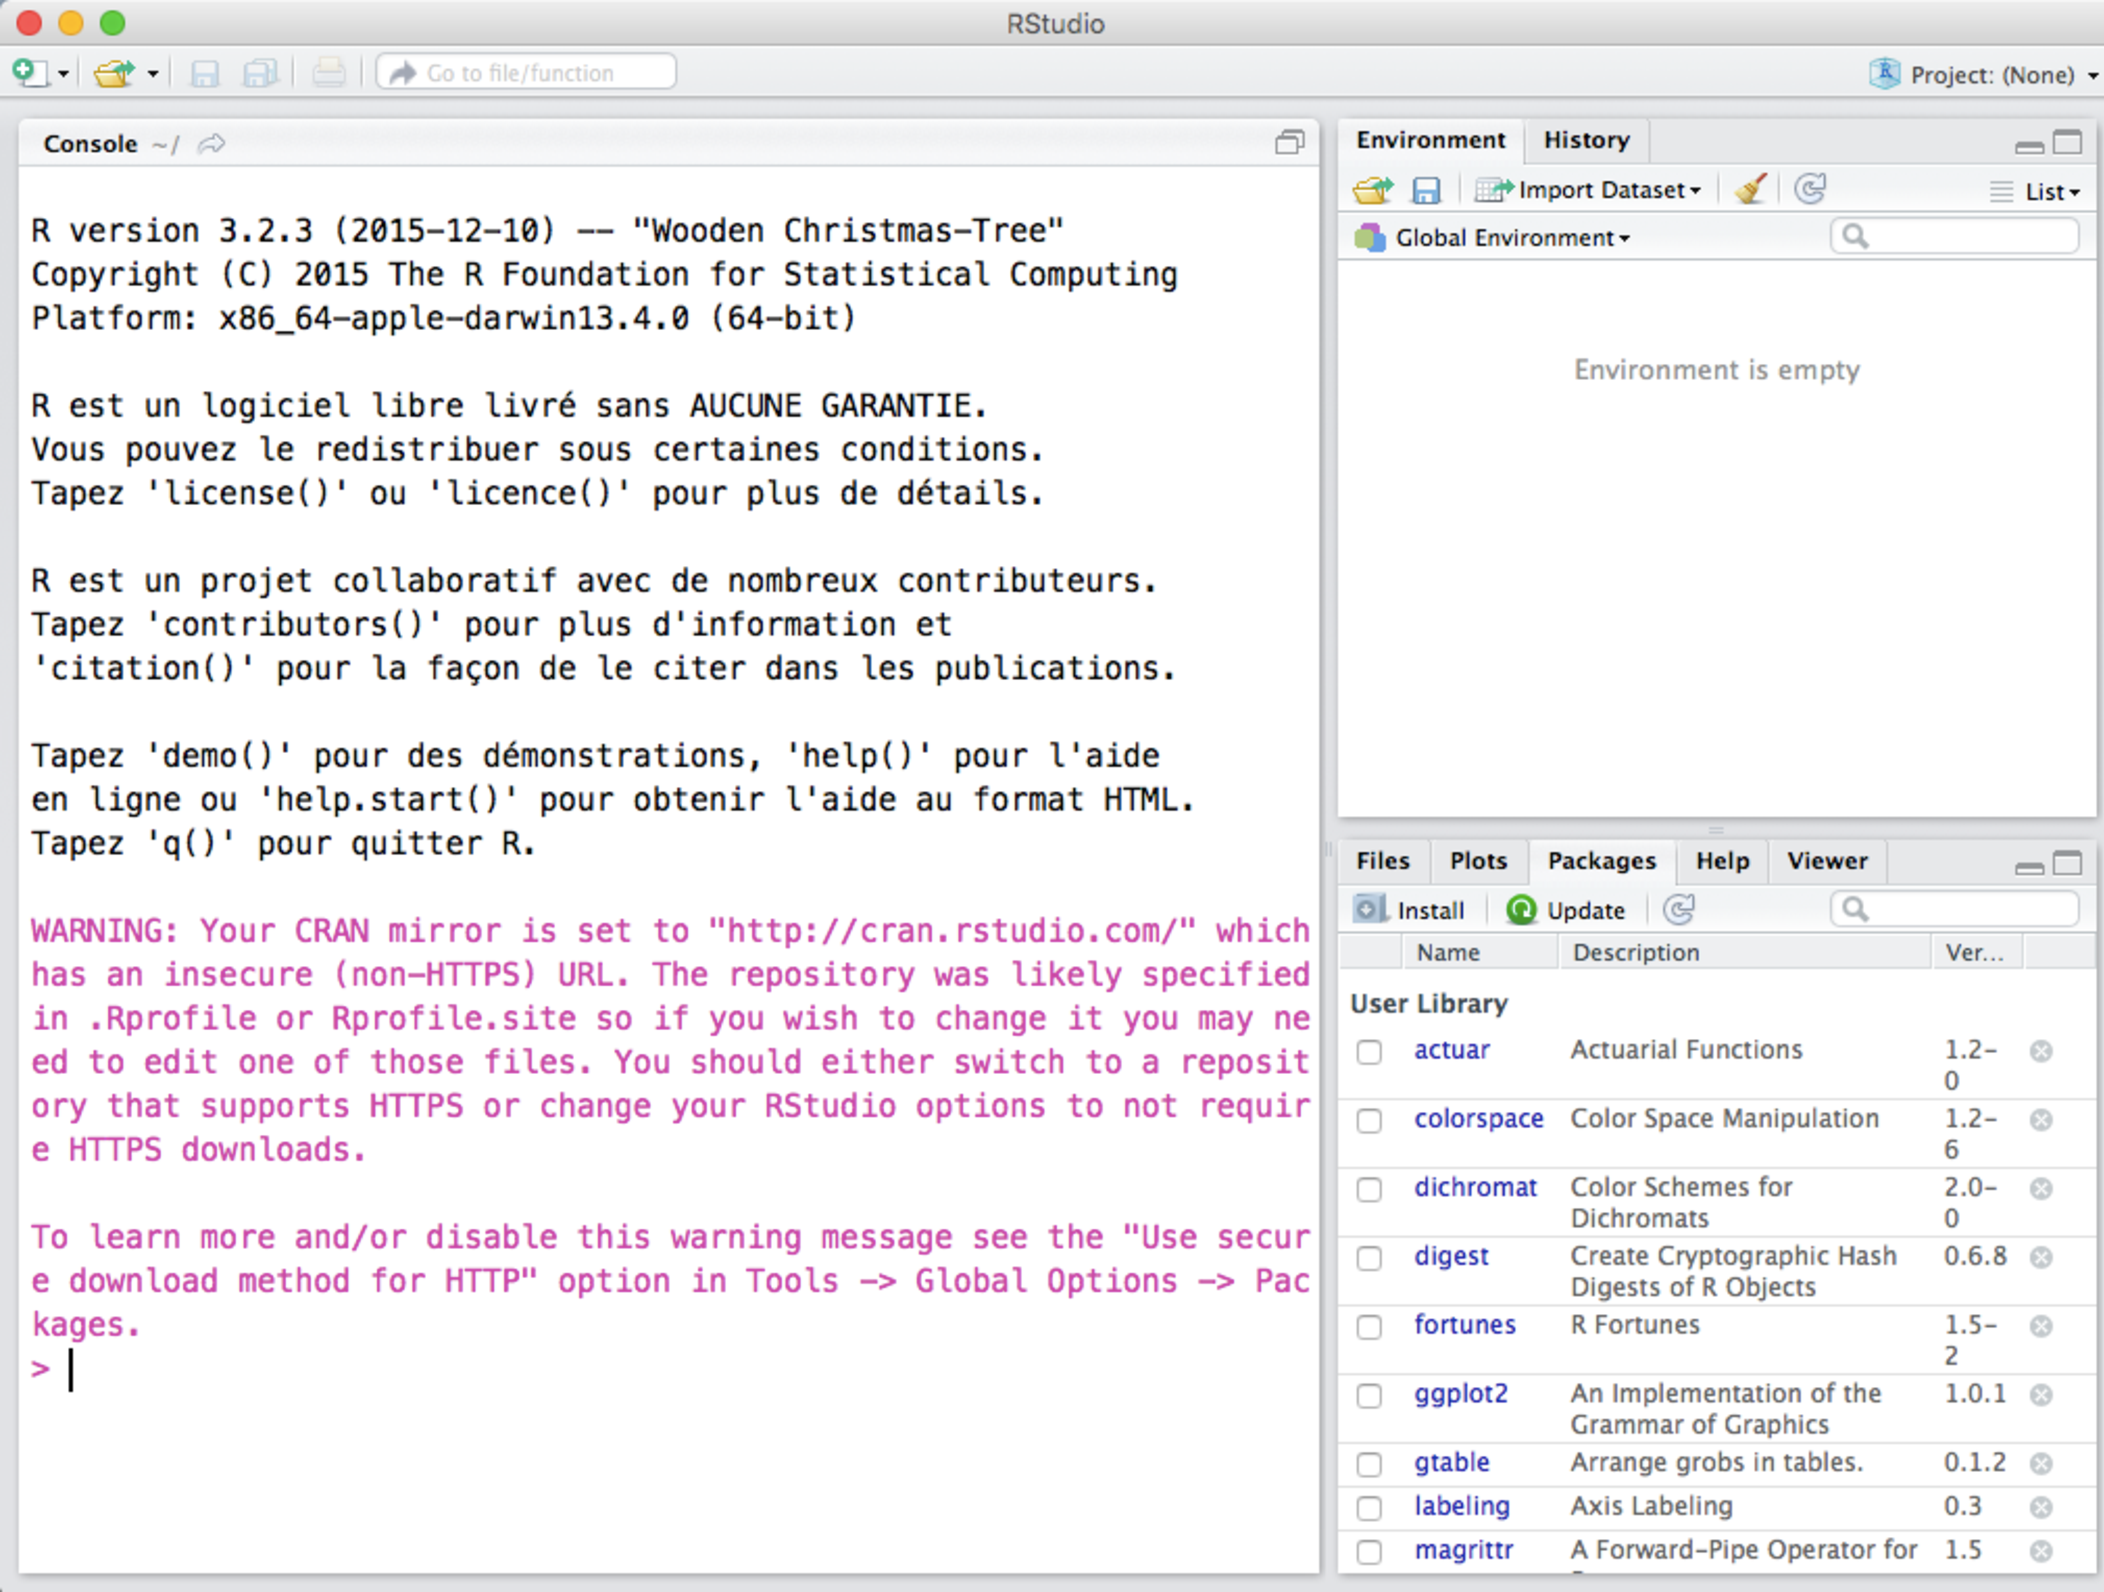
\includegraphics{rstudiowindow-screenshot}
  \vspace{0.5\TPVertModule}

  %% Identification de la console
  \begin{textblock}{0.5}(2.65,-0.62)
    \large\faLongArrowDown
  \end{textblock}
  \begin{textblock}{2}(2.2,-0.3)
    \footnotesize\sffamily Console R
  \end{textblock}

  %% Identification du navigateur d'environnement
  \begin{textblock}{1}(7.52,-3.65)
    \large\faLongArrowRight
  \end{textblock}
  \begin{textblock}{2.2}(7.95,-3.9)
    \footnotesize\sffamily\raggedright Navigateur d'environnement et d'historique
  \end{textblock}

  %% Identification de navigateur de fichiers
  \begin{textblock}{1}(7.52,-1.65)
    \large\faLongArrowRight
  \end{textblock}
  \begin{textblock}{2.2}(7.95,-1.9)
    \footnotesize\sffamily\raggedright Navigateur de fichiers, packages, graphiques, etc.
  \end{textblock}
  \caption{Fenêtre de RStudio et ses différentes parties au lancement
    de l'application sous Mac OS~X. Sous Windows et Linux, la barre de
    menu se trouve à l'intérieur de la fenêtre.}
  \label{fig:rstudio:rstudiowindow}
\end{figure}


\section{Projets}
\label{sec:rstudio:projets}

Il est possible d'utiliser RStudio un peu comme un simple éditeur de
texte.
\begin{itemize}
\item On ouvre les fichiers de scripts un à un, soit à partir du menu
  \code{File|Open file...}, soit à partir de l'onglet \code{Files} du
  navigateur de fichiers.
\item Une seule session R est alors active.
\item Lorsque nécessaire, on change le répertoire de travail de R à
  partir du menu \code{Session}.
\end{itemize}

La véritable puissance de RStudio pour l'organisation de son travail
réside cependant dans l'utilisation de \emph{projets}.
\begin{itemize}
\item Un projet RStudio est associé à un répertoire de travail de R
  (\autoref{presentation:workspace}).
\item On crée un nouveau projet à partir du menu \code{Project} à
  l'extrémité droite de la barre d'outils ou à partir du menu
  \code{File|New Project...} On a alors l'option de créer un nouveau
  dossier sur notre poste de travail ou de créer un projet à partir
  d'un dossier existant.
\item Lors de la création d'un projet, RStudio crée dans le dossier
  visé un fichier avec une extension \code{.Rproj} contenant diverses
  informations en lien avec le projet. De plus, le projet est
  immédiatement chargé dans RStudio.
\item L'ouverture d'un projet entraîne également le lancement d'une
  \emph{nouvelle} session R ayant comme répertoire de travail le
  dossier du projet, le chargement du fichier \code{.RData} (le cas
  échéant) et l'ouverture de tous les fichiers de scripts qui étaient
  ouverts lors de la dernière séance de travail.
\item Il est possible de travailler sur plusieurs projets en même
  temps.
\item Chaque projet dispose de ses propres réglages. On accède à
  ceux-ci via la commande \code{Project Options...} du menu
  \code{Project} de la barre d'outils.
\end{itemize}

On peut se donner cette règle de fonctionnement: si un projet, un
travail, un cours mérite son propre dossier sur son poste de travail,
alors l'environnement R afférant mérite son projet dans RStudio.

On trouvera plus d'information sur les projets dans l'aide en ligne
de RStudio.

\begin{important}
  L'utilisation de projets constitue la manière la plus simple et la
  plus intuitive de démarrer plusieurs sessions R dans RStudio avec
  chacune son propre répertoire de travail. Leur utilisation est donc
  fortement recommandée.
\end{important}


\section{Commandes de base}
\label{rstudio:commandes}

L'interface de RStudio étant conforme aux standards des applications
modernes, nous ne soulignons ici que les commandes particulièrement
utiles pour la manipulation des fichiers de script. On accède
rapidement à la liste des commandes les plus utiles via le menu
\code{Help} de l'application.

On fournit ci-dessous les raccourcis clavier d'abord sous Windows et
Linux, puis sous OS~X.

\begin{ttscript}{Ctrl-Shift-S $\bullet$ \cmdkey\shiftkey S}
  \raggedright
\item[\rstudio{Alt+-} $\bullet$ \rstudio{\optkey\,-}] insérer le
  symbole d'assignation \verb*| <- |
\item[\rstudio{Ctrl+Retour} $\bullet$ \rstudio{\cmdkey\,\returnkey}]
  évaluer dans le processus R la ligne sous le curseur ou la région
  sélectionnée, puis déplacer le curseur à la prochaine expression
\item[\rstudio{Ctrl+Shift+S} $\bullet$ \rstudio{\shiftkey\,\cmdkey\,S}]
  évaluer le code du fichier courant en entier dans le processus R
\item[\rstudio{Ctrl+Alt+B} $\bullet$ \rstudio{\optkey\,\cmdkey\,B}]
  évaluer dans le processus R le code source du début du fichier
  jusqu'à la ligne sous le curseur
\item[\rstudio{Ctrl+Alt+E} $\bullet$ \rstudio{\optkey\,\cmdkey\,E}]
  évaluer dans le processus R le code source de la ligne sous le curseur
  jusqu'à la fin du fichier
\item[\rstudio{Ctrl+Alt+F} $\bullet$ \rstudio{\optkey\,\cmdkey\,F}]
  évaluer le code de la fonction courante dans le processus R
\end{ttscript}

À la console --- ou ligne de commande --- R, les raccourcis suivants
sont particulièrement utiles.
\begin{ttscript}{Ctrl-I $\bullet$ \cmdkey\,I}
  \raggedright
\item[$\uparrow$ | $\downarrow$] expression
  précédente~|~suivante dans l'historique des commandes
\item[\code{Ctrl+}$\uparrow$ $\bullet$ \cmdkey\,$\uparrow$] afficher
  la fenêtre d'historique des commandes
\end{ttscript}

\begin{figure}[t]
  \begin{osx}
    Le très pratique raccourci clavier {\optkey\,-} servant à insérer
    le symbole d'assignation ne fonctionne pas avec le clavier
    canadien français puisque cette combinaison de touches sert déjà à
    insérer le symbole \textbar.

    Au moment d'écrire ces lignes, RStudio ne permet pas de réaffecter
    la commande d'insertion du symbole d'assignation à une autre combinaison de touches.

    Une solution de rechange consiste à utiliser une disposition de
    clavier anglaise pour travailler dans RStudio.

    Pour ce faire, accéder aux préférences système de OS~X puis
    sélectionner l'option Clavier. Dans l'onglet Méthodes de saisie,
    installer un nouveau clavier Anglais. Cocher l'option «Afficher le
    menu de saisie dans la barre des menus» pour pouvoir rapidement et
    facilement changer de clavier.
  \end{osx}
  \label{fig:rstudio:assignation}
\end{figure}


\section{Anatomie d'une session de travail (bis)}
\label{rstudio:session}

On reprend ici les étapes d'une \capsule{http://youtu.be/xiNnHegDau8}{session de
  travail} type présentées à la \autoref{presentation:session}, mais
en expliquant comment compléter chacune dans RStudio.

\begin{enumerate}
\item Lancer l'application RStudio.
\item
\item Démarrer un processus R à l'intérieur même de Emacs avec
  \begin{quote}
    \code{M-x R }\returnkey
  \end{quote}
  Emacs demandera alors de spécifier de répertoire de travail
  (\emph{starting data directory}). Accepter la valeur par défaut, par
  exemple
  \begin{quote}
    \verb=~/ =\returnkey
  \end{quote}
  ou indiquer un autre dossier. Un éventuel message de Emacs à l'effet
  que le fichier \code{.Rhistory} n'a pas été trouvé est sans
  conséquence et peut être ignoré.
\item Composer le code. Lors de cette étape, on se déplacera souvent
  du fichier de script à la ligne de commande afin d'essayer diverses
  expressions. On exécutera également des parties seulement du code se
  trouvant dans le fichier de script. Les commandes les plus utilisées
  sont alors
  \begin{quote}
    \ess{C-RET}\ pour exécuter une ligne du fichier de script; \\
    \ess{C-c C-c}\ pour exécuter un paragraphe du fichier de script; \\
    \emacs{C-x o}\ pour se déplacer d'une fenêtre à l'autre; \\
    \ess{C-c C-e}\ pour replacer la ligne de commande au bas de la
    fenêtre.
  \end{quote}
\item Sauvegarder le fichier de script:
  \begin{quote}
    \emacs{C-x C-s}
  \end{quote}
  Les quatrième et cinquième caractères de la ligne de mode changent
  de \,\verb|**|\, à \,\verb|--|.
\item Sauvegarder si désiré l'espace de travail de R avec
  \code{save.image()}\indexfonction{save.image}. On le répète, cela
  n'est habituellement pas nécessaire à moins que l'espace de travail
  ne contienne des objets importants ou longs à recréer.
\item Quitter le processus R avec
  \begin{quote}
    \ess{C-c C-q}
  \end{quote}
  Cette commande ESS se chargera de fermer tous les fichiers associés
  au processus R. On peut ensuite quitter Emacs en fermant
  l'application de la manière usuelle.
\end{enumerate}



\section{Configuration de l'éditeur}
\label{rstudio:configuration}



\section{Aide et documentation}
\label{rstudio:aide}


%%% Local Variables:
%%% mode: latex
%%% TeX-master: "introduction_programmation_r"
%%% coding: utf-8
%%% End:
